\section{Результаты работы шестой лабораторной работы}

\subsection{О COCOMO}

Цель: ознакомление с существующими методиками предварительной оценки параметров программного проекта и практическая оценка затрат на примере методики COCOMO (COnstructive COst MOdel — конструктивная модель стоимости).

COCOMO (COnstructive COst MOdel) –-- одна из основных методик, которые применяются для оценки стоимости ПО, отличается простотой расчётов. 

 
С1 --- масштабируемый коэффициент.

EAF --- уточняющий фактор, характеризующий предметную область, персонал, среду и инструментарий, используемый для создания рабочих продуктов процесса. 

Размер --- размер конечного продукта (кода, созданного человеком), измеряемый в исходных инструкциях, которые необходимы для реализации требуемой функциональной возможности.

P1 --- показатель степени, характеризующий экономию при больших масштабах, присущую тому процессу, который используется для создания конечного продукта; в частности, способность процесса избегать непроизводительных видов деятельности (доработок, бюрократических проволочек, накладных расходов на взаимодействие).

 
С2 --- масштабирующий коэффициент для сроков исполнения.

Р2 --- показатель степени, который характеризует инерцию и распараллеливание, присущие управлению разработкой ПО.

Выделяется 3 режима модели:

Обычный (меньше 50 тысяч строк) – некрупный проект, небольшая команда, нет нововведений, всё хорошо знакомо
Промежуточный (от 50 до 500 тысяч строк) – проект среднего размера, необходимы небольшие инновации
Встроенный (более 500) – большая команда, большой проект, значительный объем инноваций, нестабильные элементы.
COCOMO рассчитывает трудоёмкость разработки как функцию от размера программы и множества факторов, каждый из которых имеет свой вес.


\begin{figure}[ht!]
	\includegraphics[width=0.75\linewidth]{assets/images/Значение драйверов затрат.png}
	\label{fig:r2}
	\caption{Значение драйверов затрат}
\end{figure}
\FloatBarrier

Каждому из факторов может находиться на одном из 6 уровней (по значению или важности фактора).

Преимущества COCOMO:

\begin{enumerate}
	\item универсальный метод;
	\item поддержка разных режимов и уровней разработки;
	\item коэффициенты получены на большом корпусе проектов;
	\item хорошая документация;
\end{enumerate}

Недостатки COCOMO:

\begin{enumerate}
	\item все уровни зависят от оценки размера проекта;
	\item не учитывается изменяемость требований;
	\item не учитывается возможность повторного использования кода, итерационные возвраты по этапам жизненного цикла, ООП;
	\item поверхностное внимание безопасности и надёжности;
\end{enumerate}

\subsection{Задание 1}

Исследовать влияние характеристик атрибутов программного проекта (MODP, TOOL) 
на трудоемкость (РМ) и время разработки проекта (ТМ) для базового уровня модели COCOMO и разных типов проектов 
(обычного, встроенного, промежуточного).
Для этого получить значения PM и ТМ по всем типам проектов для одного и того же значения параметра SIZE (размера программного кода) 
при изменении значений атрибутов проекта от низких до высоких. Проанализировать как повлияет на трудоемкость и 
время реализации проекта внесение дополнительных ограничений на требуемые сроки разработки (параметр SCED). 
Результаты исследований оформить графически и сделать соответствующие выводы.

Результат:

\begin{figure}[ht!]
	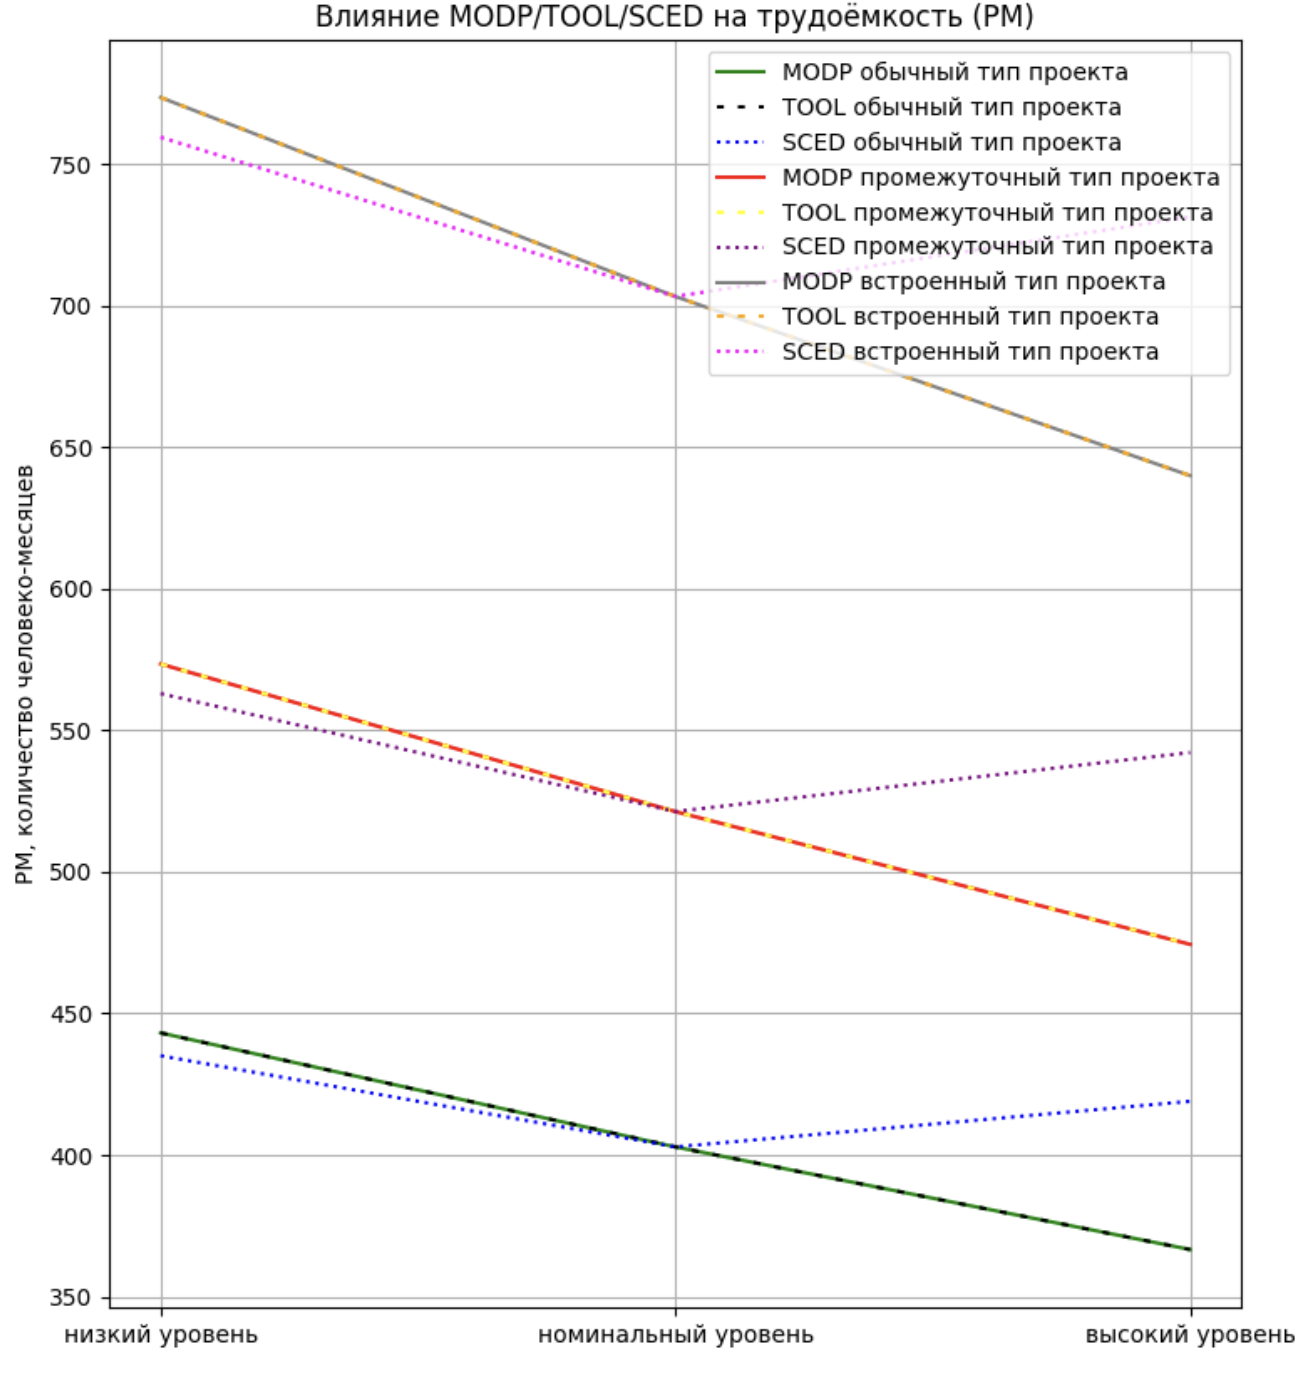
\includegraphics[width=0.75\linewidth]{assets/images/Влияние фвофажфда.png}
	\label{fig:r2}
	\caption{Результаты}
\end{figure}
\FloatBarrier

MODP – Использование современных методов

TOOL – Использование программных инструментов

SCED – Требуемые сроки разработки

\begin{figure}[ht!]
	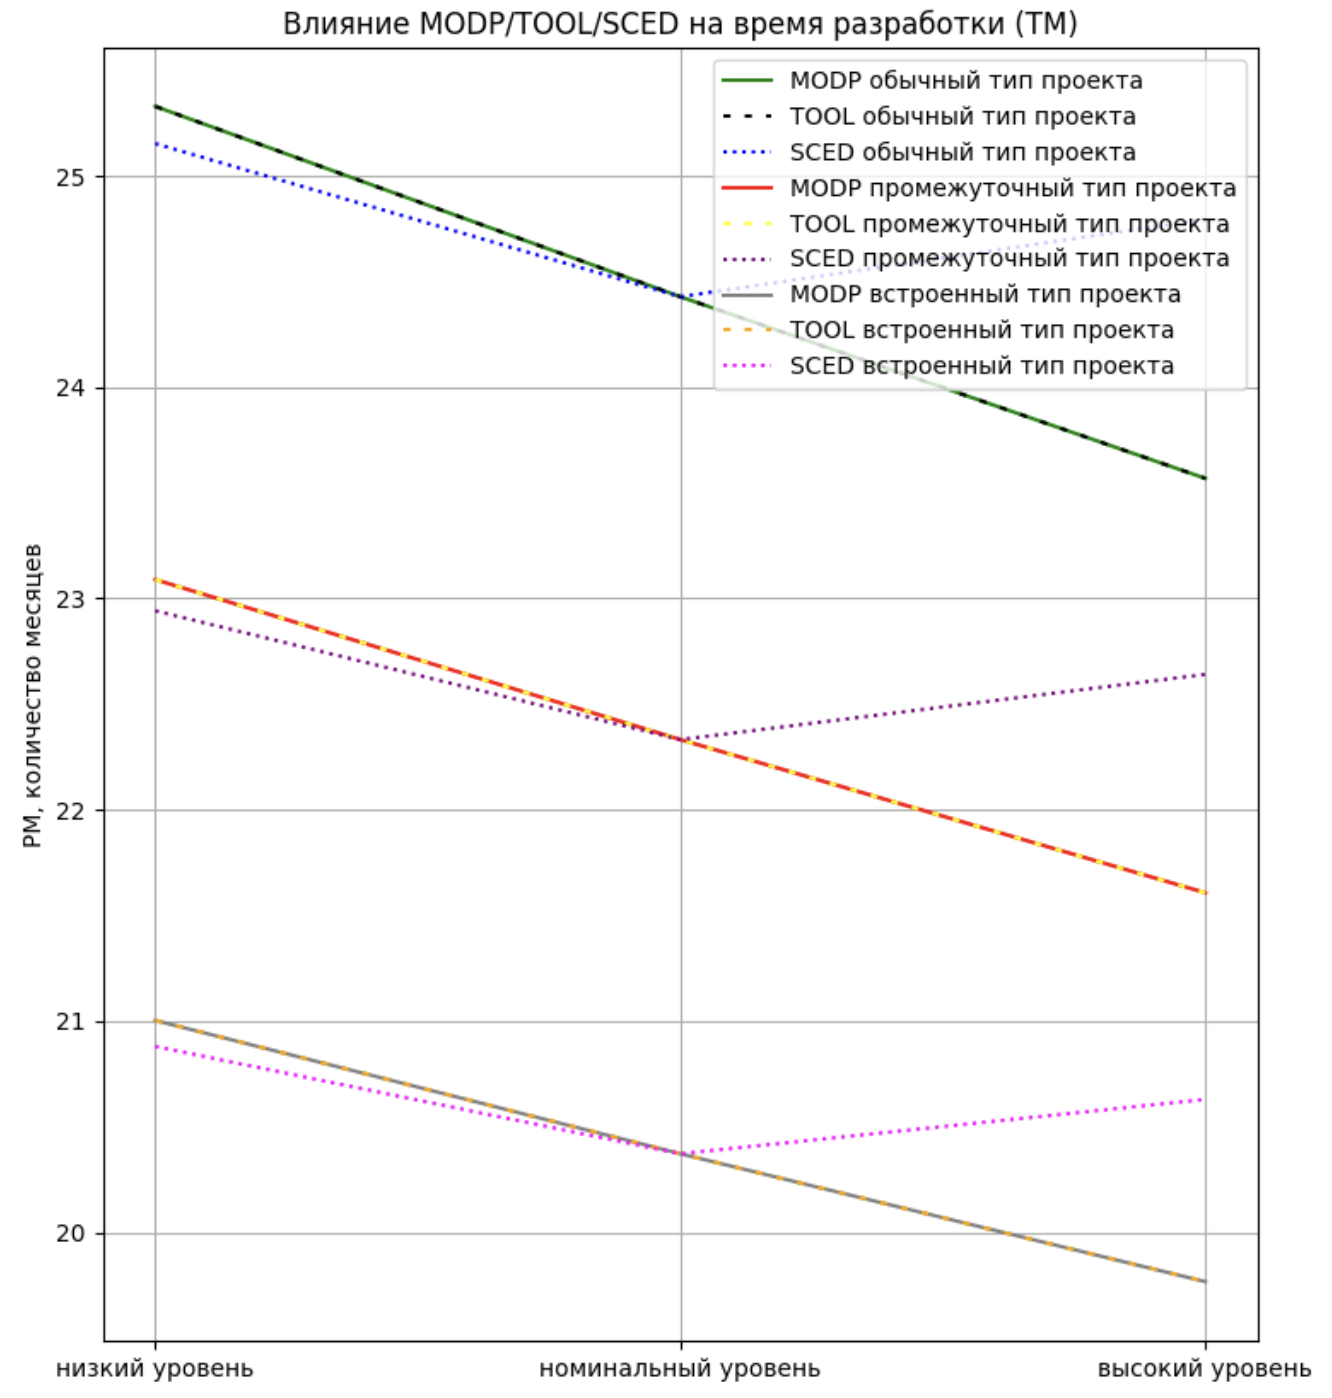
\includegraphics[width=0.75\linewidth]{assets/images/2.2 Влияние.png}
	\label{fig:r2}
	\caption{Результаты}
\end{figure}
\FloatBarrier

На графике изображены 3 группы графиков, демонстрирующих поведение для обычного, промежуточного и встроенного типов проекта. 

\begin{enumerate}
	\item На срок влияет больше что? Способности персонала (PCAP) или параметры среды (MODP) --- Для сокращения лучше подойдет наращивание способности персонала.
	\item Как и ожидалось, проекты по трудоёмкости расположились в следующем порядке: встроенный проект (самое большое значение), 
	промежуточный и обычный проект.
	\item Обратная картина наблюдается, если расположить проекты по количеству затрачиваемых месяцев. 
	Поскольку у обычного типа проекта рейтинг привлечения каких бы то ни было усовершенствований (привлечение современных методов, программных компонентов, высоких знаний у персонала) достаточно низкий, поэтому и время на разработку требуется больше.
	\item 	 Из-за того, что на всех уровнях значения величин MODP и TOOL совпадают, то, ожидаемо, эти параметры оказывают одинаковое влияние на весь процесс, поэтому графики наложены друг на друга.
	\item С увеличением привлечённости современных методов и программных продуктов трудоёмкость и время на разработку ожидаемо снижается.
	\item Сравнивая влияние на трудоёмкость в разные типы проектов, получается, что:
		\begin{itemize}
			\item наибольший «перепад» наблюдается у встроенного типа (примерно на 134 человеко-месяцев);
			\item на промежуточный тип приходится разница в 98 единиц;
			\item а на обычный – 78.
		\end{itemize}
	\item Если рассматривать время, то получается следующее:
		\begin{itemize}
			\item Наибольший перепад – 1.7 месяцев у обычного типа проекта;
			\item 1.5 – промежуточный;
			\item 1.3 – встроенный тип.
		\end{itemize}
	\item Изменяя параметр SCED (требуемые сроки разработки):
		\begin{itemize}
			\item при переходе с низкого уровня на номинальный трудоёмкость и время разработки уменьшаются, поскольку соблюдению сроков уделяется больше внимания, что позволяет снизить этот показатель;
			\item но при переходе на высокий уровень трудоёмкость резко увеличивается (а также время на выполнение), т.к. роль сроков очень высока, жесткие рамки сроков, поэтому нужно больше человеко-месяцев.
		\end{itemize}
	\item Больше влияние на трудоемкость и время выполнения влияет (RELY или TIME): RELY. (надежность)
\end{enumerate}

\subsection{Задание 2}

При разработке программного проекта его размер оценивается примерно в 55 KLOC. Этот проект будет представлять собой Webсистему, снабженную устойчивой серверной базой данных. Предполагается применение промежуточного варианта. Проект предполагает создание продукта средней сложности с номинальными требованиями по надежности, но с расширенной базой данных. Квалификация персонала средняя. Однако способности аналитика высокие. Оценить параметры проекта.

Интерфейс:

\begin{figure}[ht!]
	\includegraphics[width=0.6\linewidth]{assets/images/3.1 Интерфейс.png}
	\caption{Интерфейс}
\end{figure}
\FloatBarrier

Результат:

\begin{figure}[ht!]
	
\includegraphics[width=0.75\linewidth]{assets/images/3.2 Результат.png}
	\caption{Результат}
\end{figure}
\FloatBarrier

Без планирования показатели Трудозатрат и Времени меньше, поскольку само планирование занимает определённое время.

Таким образом, Трудозатраты составили 268 человеко-месяцев, время на выполнение проекта составляет около 24 месяцев.

Было принято, что средняя зарплата сотрудников 60 000, программист получает среднюю заплату, аналитик – в 1.4 раза больше средней, менеджер – в 1.3, а тестировщик в 0.65 меньше, чем средняя заработная плата. 

\begin{figure}[ht!]
	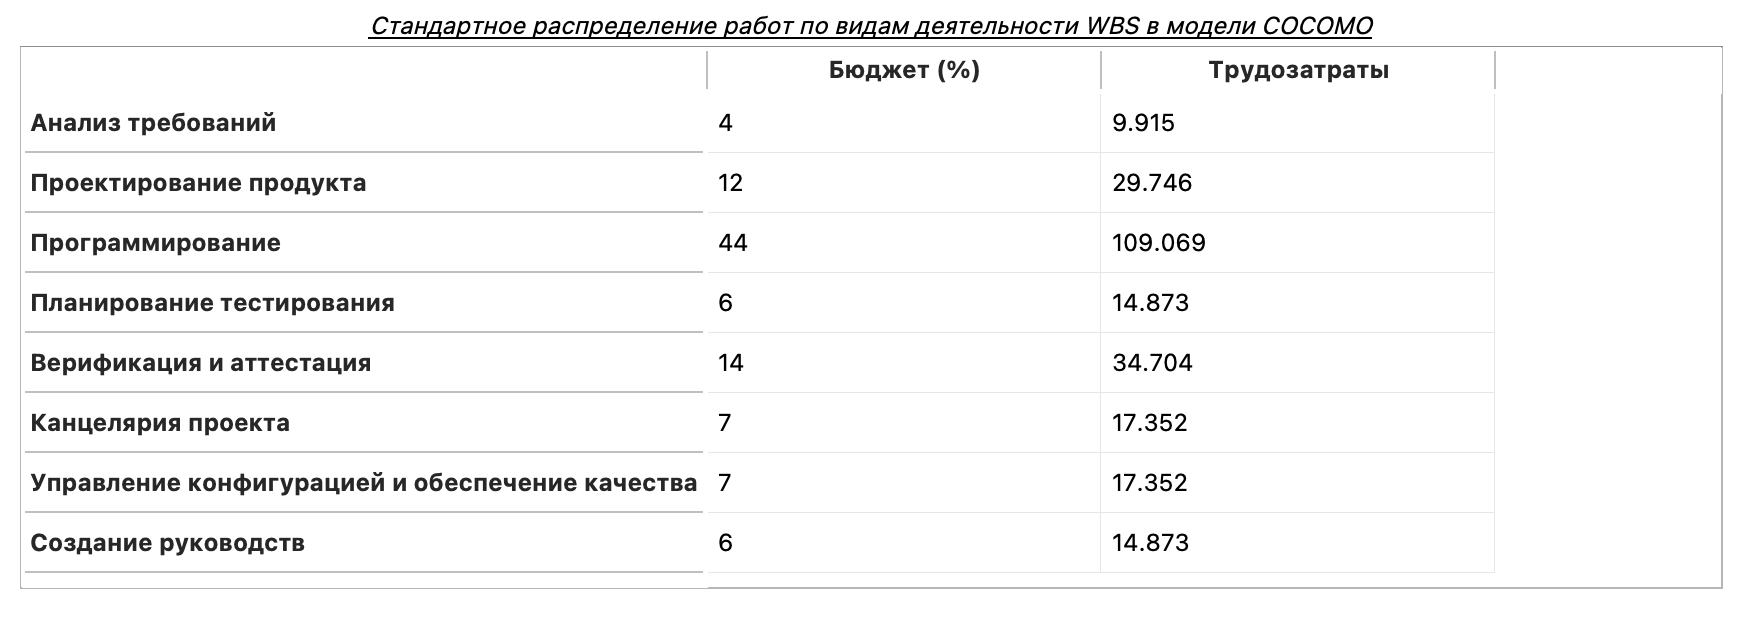
\includegraphics[width=0.75\linewidth]{assets/images/3.4 Результаты.png}
	\caption{Интерфейс}
\end{figure}
\FloatBarrier

\begin{figure}[ht!]
	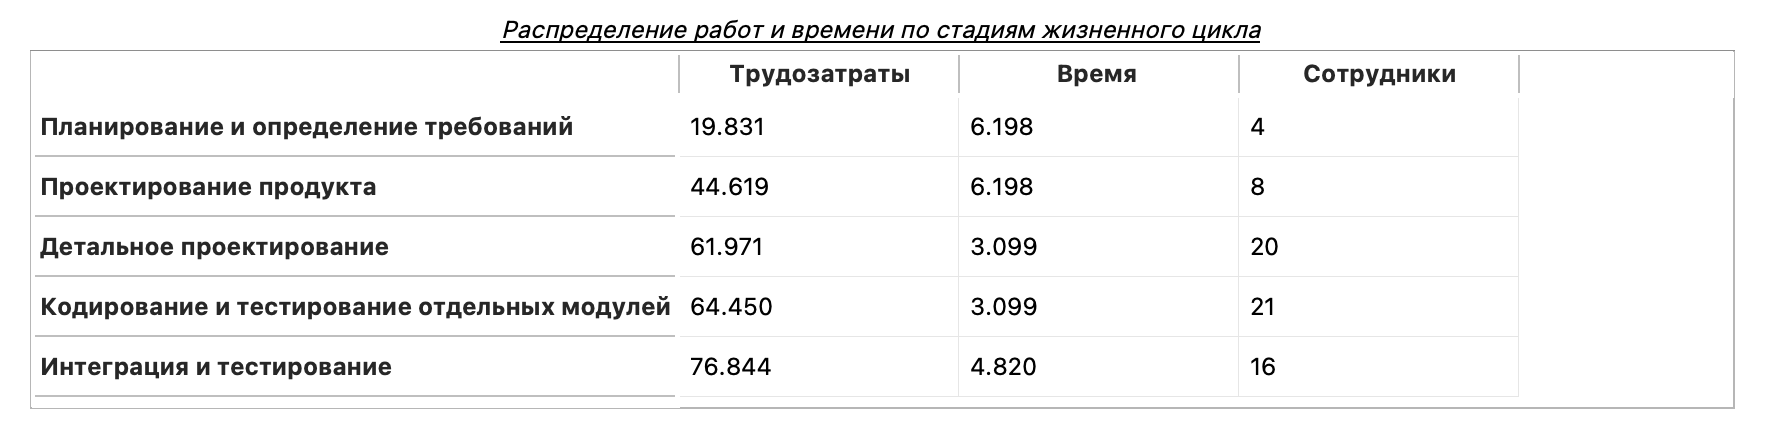
\includegraphics[width=0.75\linewidth]{assets/images/3.5 Результаты.png}
	\caption{Интерфейс}
\end{figure}
\FloatBarrier

Были получены распределения работ и времени по стадиям жизненного цикла и по видам деятельности. Количество сотрудников определялось как частное от трудозатрат и времени, округлённое в большую сторону.

По стадиям жизненного цикла наблюдается следующее:

\begin{enumerate}
	\item наибольшие трудозатраты требует интеграция и тестирование, однако по времени этот процесс не является самым продолжительным;
	\item на втором месте по трудозатратам находится кодирование и тестирование отдельных модулей, но времени затрачивается еще меньше, чем на интеграцию, но на этот этап приходится наибольшее количество сотрудников;
	\item также много сотрудников (разница в 1 человека) требуется привлечь на детальное проектирование, этот этап занимает третье место по трудозатратам;
	\item больше всего времени уделяется планированию и определению требований, и проектированию продукта, однако в сумме количество сотрудников, задействованных на этих этапах меньше, чем на любом другом этапе.
\end{enumerate}

По видам деятельности в модели COCOMO:

\begin{enumerate}
	\item больше всего трудозатрат приходится на программирование (44 \%);
	\item далее идут верификация и аттестация и проектирование продукта.
\end{enumerate}

\begin{figure}[ht!]
	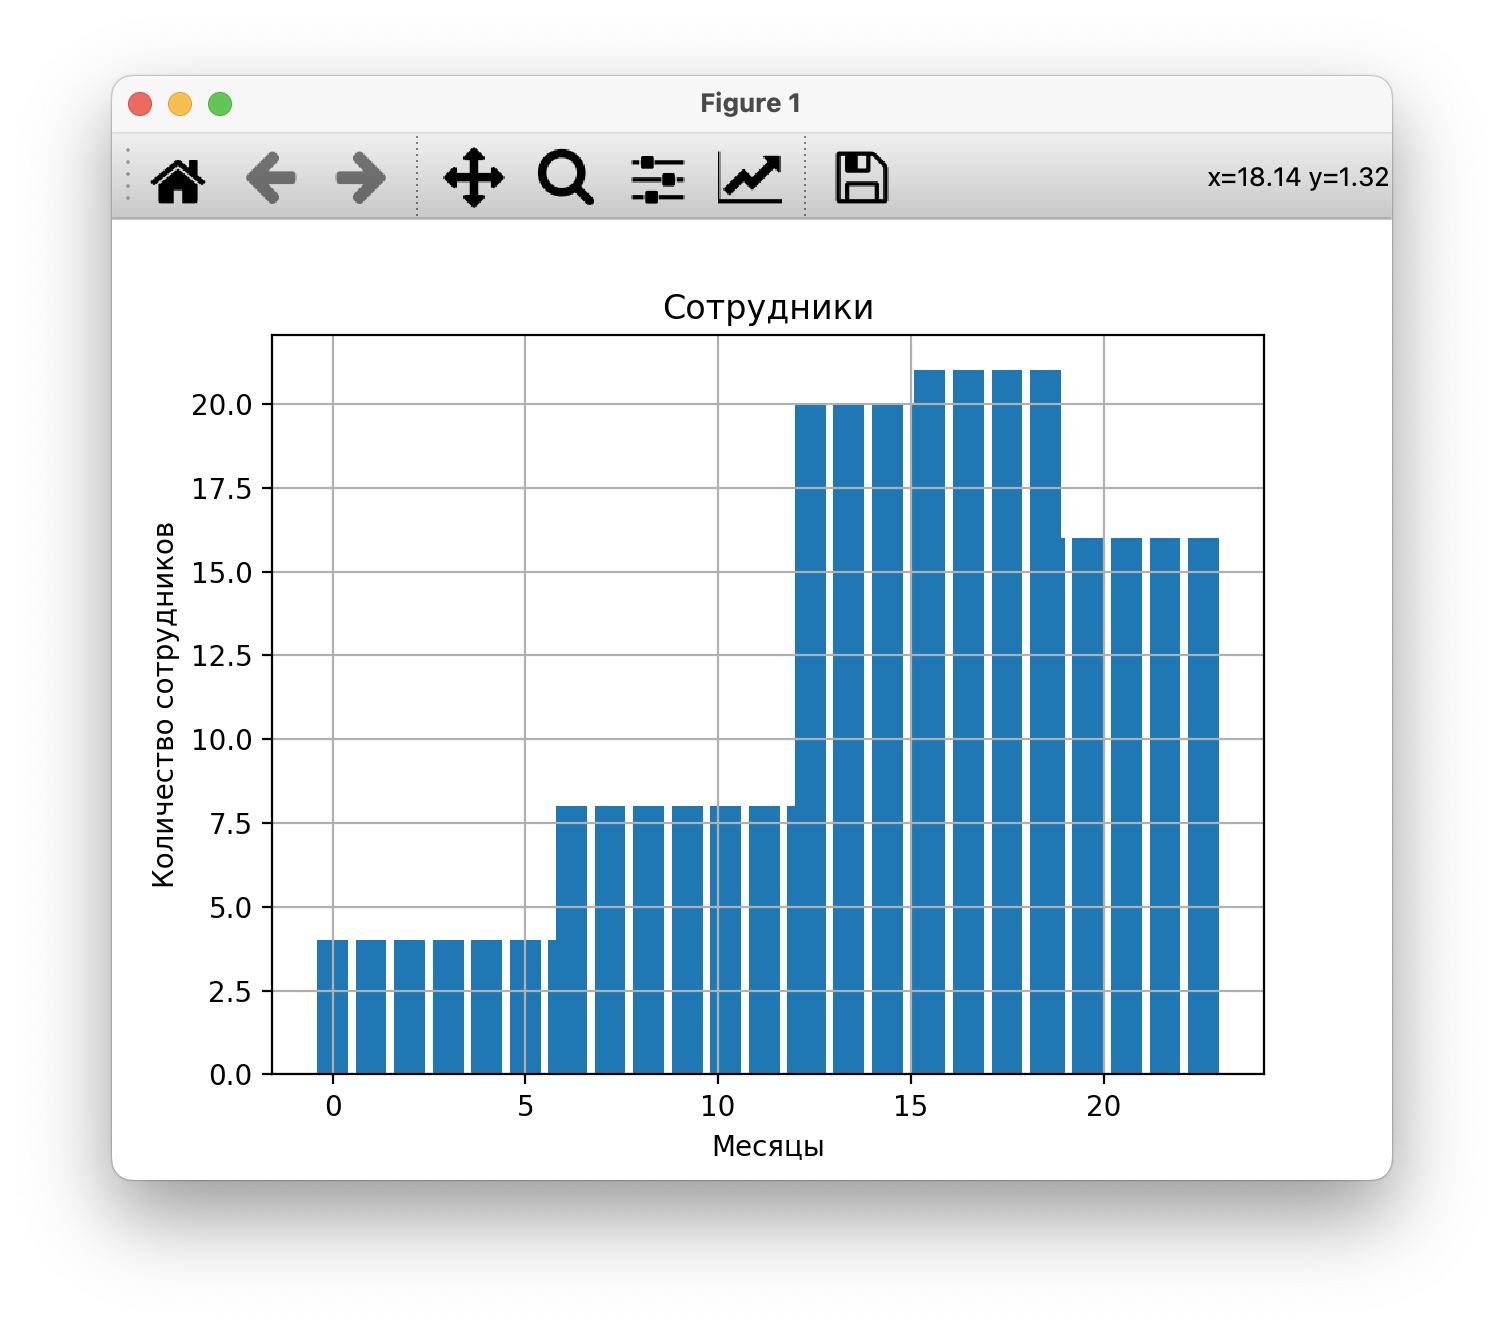
\includegraphics[width=0.6\linewidth]{assets/images/3.3 Сотрудники.png}
	\caption{Интерфейс}
\end{figure}
\FloatBarrier

Также была получена диаграмма, демонстрирующая необходимое количество работников на протяжении всего цикла создания продукта. Наибольший пик приходится на кодирование и детальное проектирование проекта.

\subsection*{Вывод}

Метод COCOMO позволяет дать первичную оценку проекта, используя знания о количестве строк кода проекта. Также возможно, варьируя значения факторов, оказывающих влияние на ход проекта, получить более точную оценку. Однако этот подход не учитывает такие важные факторы, как повторное использование кода, что может в свою очередь снизить трудозатраты и время, также мало внимания уделяется обеспечению безопасности и надёжности продукта.

Касаемо текущего проекта: 

трудозатраты --- 268 человеко-месяцев;

время --- 24 месяца.

бюджет --- 14873080.347